\section{Background}
DeltaRCM \cite{Liang2015a,Liang2015} is a proven \cite{Liang2015,Liang2016a} and popular \cite{Liang2016,Lauzon2018, Lauzon2019,Piliouras2021} numerical model used to simulate river delta growth and evolution.
The original model was written in MATLAB \cite{MATLAB:R2019b_u4}, leaving room for improvement with regards to code accessibility, run-time, documentation, parallelization, and extensibility.
With these needs in mind, a Python \cite{PythonSoftwareFoundation2016} implementation of the original DeltaRCM model was developed, dubbed \textit{pyDeltaRCM} \cite{Moodie2021}.
This re-implementation of the DeltaRCM model includes minor modifications to the original DeltaRCM methods, and so there is a need to compare the new \textit{pyDeltaRCM} model outputs to those from the original DeltaRCM code. 
In this chapter, this model-to-model comparison is performed using a suite of 35 model runs from each version of DeltaRCM.
The similarities and differences between the two models are quantitatively assessed using a small collection of metrics.

\section{Modeled Scenarios}
Seven scenario are modeled to simulate 200 years of river delta growth into an empty basin assuming 10 bankfull days of discharge per year.
For each scenario, 5 replicate runs are conducted to capture the range of stochastic variability present due to the random walk-based methodology.

\subsection{Parameter Set}
A comprehensive although non-exhaustive list of the model parameter values used for both the MATLAB and Python simulations is provided in Table \ref{tab:params}.

\begin{table}[!ht]
\begin{center}
\begin{tabular}{| c | c | c | c | c |}
\hline
Parameter & Value \\
\hline
dx & 50 m \\
L0 & 150 m \\
Np\_water & 2000 \\
Np\_sed & 2000 \\
u0 & 1 m/s \\
N0 & 250 m \\
h0 & 5 m \\
H\_SL & 0 m \\
f\_bedload & 0.2 \\
C0\_percent & 0.1 \\
Csmooth & 0.9 \\
omega\_sfc & 0.1 \\
omega\_flow & 0.9 \\
Nsmooth & 10 \\
theta\_water & 1 \\
coeff\_theta\_sand & 2 \\
coeff\_theta\_mud & 1 \\
beta & 3 \\
sed\_lag (lambda) & 1 \\
coeff\_U\_dep\_mud & 0.3 \\
coeff\_U\_ero\_mud & 1.5 \\
coeff\_U\_ero\_sand & 1.05 \\
alpha & 0.1 \\
\hline
\end{tabular}
\caption{Model Parameters}
\label{tab:params}
\end{center}
\end{table}

The 7 modeled scenarios simulate different levels of steady sea level rise (SLR).
These 7 SLR values are 0, 5, 10, 15, 20, 30, and 40 mm/yr.
Rates of SLR are scaled temporally under the assumption that the model is simulating 10 bankfull days of discharge per year.

A low value for \texttt{f\_bedload} (20\% sand) is used in these simulations as low sand content generates highly cohesive and more variable simulation results.
High input sand fraction values will result in simulations with smoother deltas.
For the purposes of comparing models, it should be easier to detect differences between rougher planform shapes than smooth ones.


\subsection{Parameter Differences}
The interval at which model outputs are saved was different between the models. For the MATLAB code, saving occurs every 25 model timesteps, whereas in the Python code the model is saved every 35 timesteps.
The save interval does not impact the model behavior, but rather our ability to observe what the model is doing.

The modeled domain size is different between the two sets of runs performed, although in neither case do the simulated deltas reach the domain boundaries.
In the MATLAB scenarios the basin is 9 km long and 17 km wide.
In the Python scenarios the basin is slightly larger with a length of 10 km and a width of 20 km.

Two model parameters are set to slightly different values in these sets of model runs.
The reference slope, \texttt{S0}, is $1.4 \times 10^{-4}$ for the MATLAB model runs, and $1.5 \times 10^{-4}$ for the Python model runs.
The number of times the water parcel routing occurs per timestep, \texttt{itermax}, differs between the runs.
In the MATLAB models \texttt{itermax} $=1$, as this is a computationally expensive step because the water parcels are routed in serial.
The Python models use \texttt{itermax} $=3$, as the new version of the model now routes all of the water parcels in parallel making this step much faster. 

\section{Topographies}
Topography at the end of model runs (after 200 years), is shown in Figure \ref{fig:finaltopo}.
A break in the colorbar to distinguish between water and land is made at 0.5 m below sea level based on color palettes used in previous studies \cite{Liang2016a, Liang2016}.

\begin{figure}[!ht]
	\makebox[\textwidth][c]{
	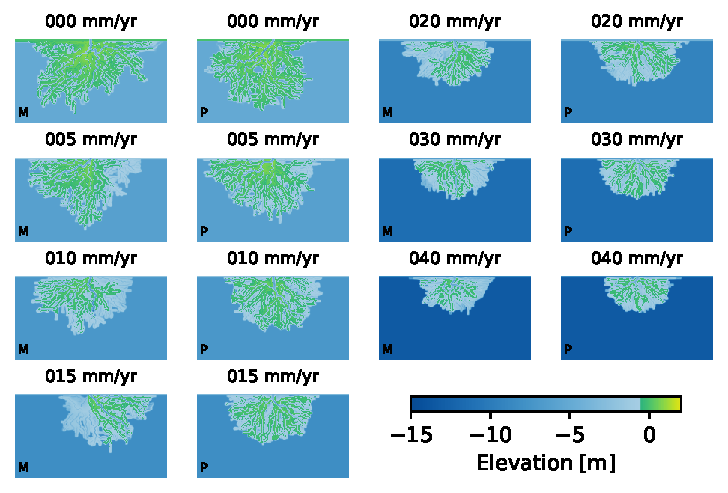
\includegraphics[width=\textwidth]{DeltaRCM_ModelComparison/figs/FinalTopo.pdf}
	}
	\caption{Single model realization final topographies. Numerical model used indicated by letter in bottom left corner of each plot, M for MATLAB and P for Python. Note that the domain has been clipped in all images.}
	\label{fig:finaltopo}
\end{figure}

\section{Metrics}

\subsection{Surface Morphology}

\subsubsection{Planform Area}
The area of the delta planform is identified using a topographic threshold of 0.5 m below the sea level \cite{Liang2016a,Liang2016} and the opening angle method \cite{Shaw2008} with an opening angle of $75^{\circ}$.

\begin{figure}[!htbp]
	\makebox[\textwidth][c]{
	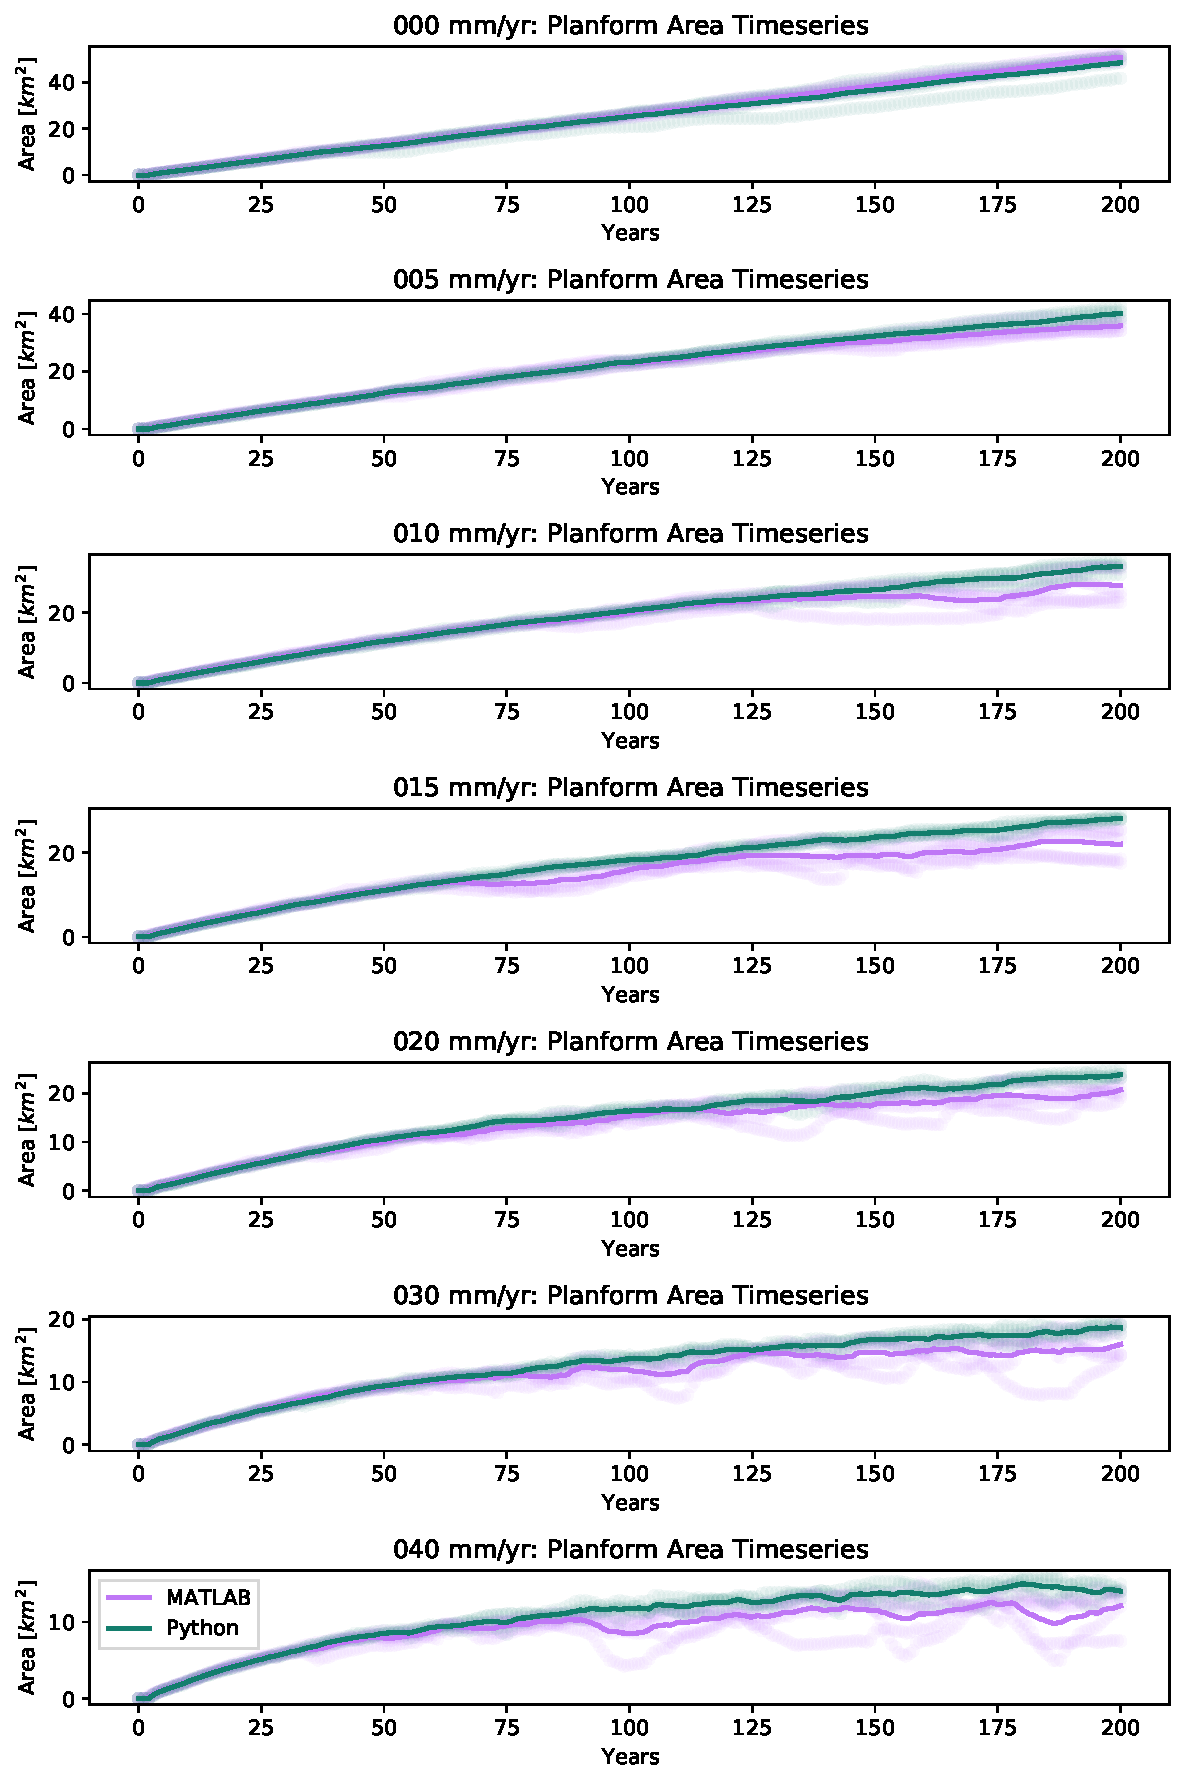
\includegraphics[height=\textheight]{DeltaRCM_ModelComparison/figs/Area.pdf}
	}
	\caption{Planform area timeseries with average values shown as lines and individual run results shown as faint circles. MATLAB results shown in light purple, Python results in dark green.}
	\label{fig:area}
\end{figure}

\subsubsection{Channelized Fraction}
The channelized pixels on the delta topset are identified as locations where the water velocity exceeds the threshold for sediment mobilization (0.3 m/s) \cite{Liang2016a,Liang2016,Lauzon2018,Lauzon2019}.
Then, the channelized fraction is computed by dividing the channelized area by the total area of the topset (the planform area).

\begin{figure}[!htbp]
	\makebox[\textwidth][c]{
	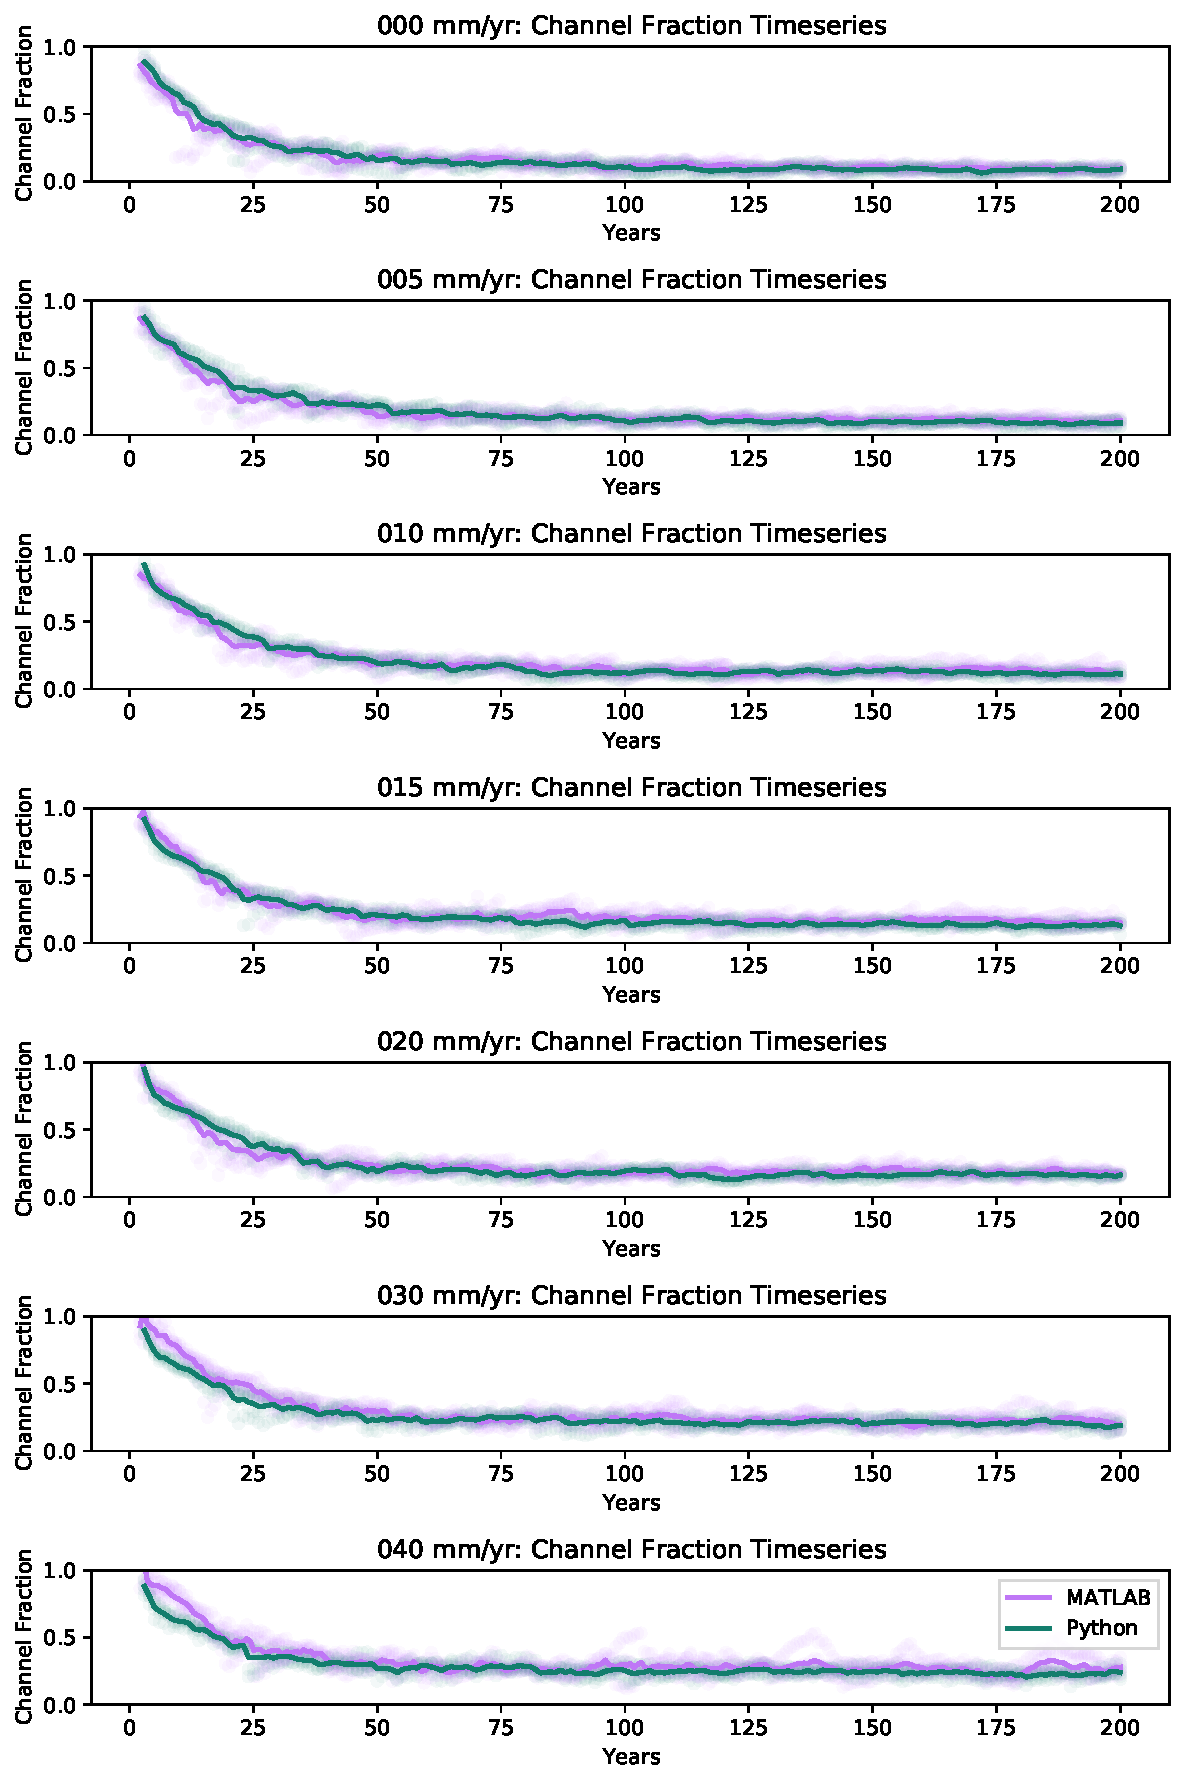
\includegraphics[height=\textheight]{DeltaRCM_ModelComparison/figs/ChannelDensity.pdf}
	}
	\caption{Channelized fraction timeseries with average values shown as lines and individual run results shown as faint circles. MATLAB results shown in light purple, Python results in dark green.}
	\label{fig:channelfraction}
\end{figure}

\subsubsection{Shoreline Roughness}
Shoreline roughness is calculated as the length of the shoreline divided by the square root of the planform area.
The shoreline is derived from the land map of the delta planform by performing morphological operations using the scikit-image Python library \cite{scikit-image}.
First edge detection \cite{roberts1963machine} is performed, and then the resulting edge is made binary and skeletonized \cite{zhang1984fast}, defining the shoreline.

\begin{figure}[!htbp]
	\makebox[\textwidth][c]{
	\includegraphics[height=\textheight]{DeltaRCM_ModelComparison/figs/ShoreRough.pdf}
	}
	\caption{Shoreline roughness timeseries with average values shown as lines and individual run results shown as faint circles. MATLAB results shown in light purple, Python results in dark green.}
	\label{fig:shorelineroughness}
\end{figure}

\subsection{Surface Dynamics}

\subsubsection{Channel Planform Overlap}
The channel planform overlap metric \cite{Wickert2013} measures the loss of similarity in channel locations over time.
It is common for the normalized overlap value, $O_{\Phi}$, to be used to fit an exponential decay equation
\begin{equation}
O_\Phi = \left(a_M - p_M\right) e^{-Mt} + p_M,
\end{equation}
where $M$, the decay constant (units of inverse time), is a mobility parameter describing how quickly the channel system is reworking itself.
For these 200 year simulations, the channel planform overlap is evaluated using base channel maps from recorded outputs in the interval [100, 150] years.
These base maps are compared to those within 50 years, meaning the transient maps are sourced from the interval (100, 200] years.

%\csvautotabular{tables/MATLAB_mobilitydata.csv}

\begin{table}[!ht]
\begin{center}
\begin{tabular}{| c | c | c | c |}
\hline
SLR [mm/yr] & $a_M$ & $M$ [yr$^{-1}$] & $p_M$ \\
\hline
\hline
\csvreader[late after line=\\\hline]
   {DeltaRCM_ModelComparison/tables/MATLAB_mobilitydata.csv}{SLR [mm/yr]=\slr, $a_M$=\am, $M$=\m, $p_M$=\pm}
   {\slr & \am & \m & \pm}
\end{tabular}
\caption{MATLAB planform overlap exponential fit parameters. Average parameter values for the set of 5 replicate runs reported $\mypm$ the average standard deviation of the individual parameter estimates.}
\label{tab:RCMmobility}
\end{center}
\end{table}

\begin{table}[!ht]
\begin{center}
\begin{tabular}{| c | c | c | c |}
\hline
SLR [mm/yr] & $a_M$ & $M$ [yr$^{-1}$] & $p_M$ \\
\hline
\hline
\csvreader[late after line=\\\hline]
   {DeltaRCM_ModelComparison/tables/Python_mobilitydata.csv}{SLR [mm/yr]=\slr, $a_M$=\am, $M$=\m, $p_M$=\pm}
   {\slr & \am & \m & \pm}
\end{tabular}
\caption{Python planform overlap exponential fit parameters. Average parameter values for the set of 5 replicate runs reported $\mypm$ the average standard deviation of the individual parameter estimates.}
\label{tab:Pymobility}
\end{center}
\end{table}

%\subsubsection{Channel Abandonment}
%Channel abandonment is calculated using the number of channelized pixels from some base map which remain channelized at later times \cite{Liang2016}.
%To this decay curve, a harmonic function is fit \cite{Cazanacli2002}, formulated as,
%\begin{equation}
%f_{remain} = \frac{f_0}{1 + \frac{t}{t_{rw}}},
%\end{equation}
%where $t_{rw}$ represents a characteristic decay time for the abandonment of the channel.

\subsection{Subsurface Composition}

\subsubsection{Net-to-Gross Ratio}
The net-to-gross ratio of the total deposit is calculated as the sum of sand fraction values in the preserved stratigraphy divided by the total number of voxels in the stratigraphy.
Stratigraphy in both models is computed at a vertical resolution of 5 cm.

\begin{table}[!ht]
\begin{center}
\begin{tabular}{| c | c | c | c | c | c | c | c |}
\hline
SLR [mm/yr] & Run 1 & Run 2 & Run 3 & Run 4 & Run 5 & \textbf{Avg.} & Std. Dev. \\
\hline
\hline
\csvreader[late after line=\\\hline]
   {DeltaRCM_ModelComparison/tables/MATLAB_netgross.csv}{SLR [mm/yr]=\slr, Run 1=\a, Run 2=\b, Run 3=\c,
   								Run 4=\d, Run 5=\e, Avg.=\avg, Std. Dev.=\std}
   {\slr & \a & \b & \c & \d & \e & \bfseries\avg & \std}
\end{tabular}
\caption{MATLAB net-to-gross values}
\label{tab:RCMnetgross}
\end{center}
\end{table}

\begin{table}[!ht]
\begin{center}
\begin{tabular}{| c | c | c | c | c | c | c | c |}
\hline
SLR [mm/yr] & Run 1 & Run 2 & Run 3 & Run 4 & Run 5 & \textbf{Avg.} & Std. Dev. \\
\hline
\hline
\csvreader[late after line=\\\hline]
   {DeltaRCM_ModelComparison/tables/Python_netgross.csv}{SLR [mm/yr]=\slr, Run 1=\a, Run 2=\b, Run 3=\c,
   								Run 4=\d, Run 5=\e, Avg.=\avg, Std. Dev.=\std}
   {\slr & \a & \b & \c & \d & \e & \bfseries\avg & \std}
\end{tabular}
\caption{Python net-to-gross values}
\label{tab:Pynetgross}
\end{center}
\end{table}

%\subsubsection{Downstream Fining}
%To obtain some measure of the spatial partitioning of sediment within the deposit, the notion of downstream fining will be explored.

\section{Statistical Tests}

\subsection{Rank-Sum Tests}
Results for the channelized fraction and shoreline roughness metrics are qualitatively stationary in time after the initial channel network is formed (Figures \ref{fig:channelfraction} \& \ref{fig:shorelineroughness}).
The DeltaRCM channel network may form in as few as 75 years \cite{Liang2016a, Lauzon2018, Lauzon2019, Piliouras2021}.
Therefore, metric values between years 100 and 200 reflect properties of the fully developed distributary network.
Values from the 5 replicates per SLR scenario are lumped together for each model (MATLAB and Python), and used to perform a rank-sum test \cite{wilcoxon1945} with a null hypothesis, $H_0$: the two sets of values are drawn from the same distribution.

\begin{table}[!ht]
\begin{minipage}[b]{0.3\linewidth}
\centering
\begin{tabular}{| l | r |}
\hline
SLR [mm/yr] & p-value \\
\hline
\hline
\csvreader[late after line=\\\hline]
   {DeltaRCM_ModelComparison/tables/channeldensity.csv}{SLR [mm/yr]=\slr, p-value=\pv}
   {\slr & \pv}
\end{tabular}
\caption{Channel Fraction Rank-Sum Results}
\label{tab:chanfrac}
\end{minipage}\hfill
\begin{minipage}[b]{0.65\linewidth}
\centering
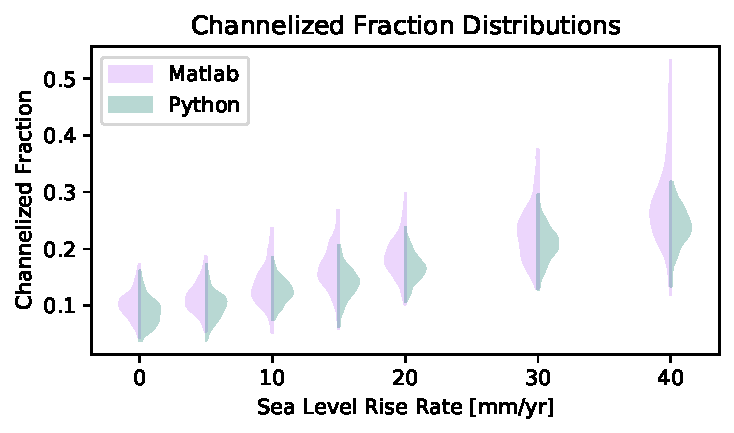
\includegraphics[width=3.5in]{DeltaRCM_ModelComparison/figs/ChannelFracDists.pdf}
\captionof{figure}{Smoothed distributions of channel fraction values (years 100-200).}
\label{fig:chanfrac}
\end{minipage}
\end{table}

\begin{table}[!ht]
\begin{minipage}[b]{0.3\linewidth}
\centering
\begin{tabular}{| l | r |}
\hline
SLR [mm/yr] & p-value \\
\hline
\hline
\csvreader[late after line=\\\hline]
   {DeltaRCM_ModelComparison/tables/shorelineroughness.csv}{SLR [mm/yr]=\slr, p-value=\pv}
   {\slr & \pv}
\end{tabular}
\caption{Shoreline Roughness Rank-Sum Results}
\label{tab:shorerough}
\end{minipage}\hfill
\begin{minipage}[b]{0.65\linewidth}
\centering
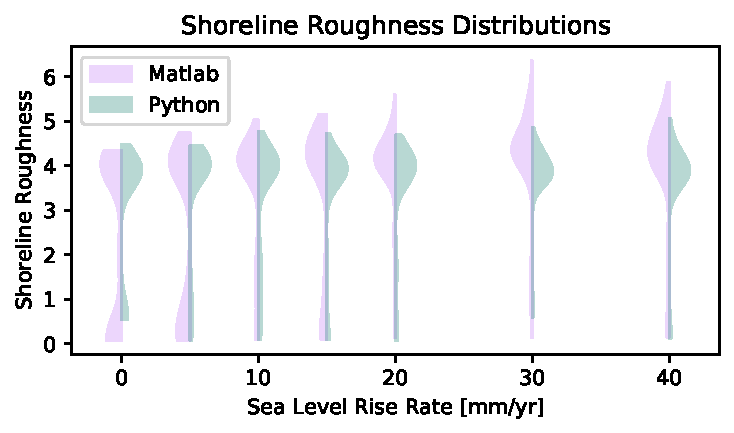
\includegraphics[width=3.5in]{DeltaRCM_ModelComparison/figs/ShoreRoughDists.pdf}
\captionof{figure}{Smoothed distributions of shoreline roughness values (years 100-200).}
\label{fig:shorerough}
\end{minipage}
\end{table}

%\subsection{Kruskal-Wallis Tests}
%Treat each individual set of results from a single model replicate as an independent group.
%Test null hypothesis that all of the 10 groups for a given scenario (5 from MATLAB, 5 from Python) have identical distributions.

\section{Conclusions}
Although model results look qualitatively very similar, there are some slight differences between the MATLAB and Python outputs.
It is hard to know whether or not these differences are due to the differences in parameter values for \texttt{S0} and \texttt{itermax}, or whether they are due to actual code differences.
It is harder still to know whether or not these differences matter and which model is generally more representative of true systems and processes.

On the surface, the channelized fraction (Figure \ref{fig:channelfraction}) and shoreline roughness (Figure \ref{fig:shorelineroughness}) appear to be similar between the models, however a rank-sum test performed comparing the values from years 100-200 (Tables \ref{tab:chanfrac} \& \ref{tab:shorerough}), suggest that the underlying distributions are indeed different.

The surface dynamics, as measured using the channel planform overlap metric, provide evidence of similar trends between the two models (increasing mobility with increasing sea level rise rates).
However, the Python implementation appears to be more mobile than the MATLAB version (Tables \ref{tab:RCMmobility} \& \ref{tab:Pymobility}, third column).
This trend in particular may be influenced by the frequency at which model outputs were obtained, the MATLAB code output information about the system every 25 timesteps ($\sim0.7$ years) whereas the Python code was set to output information every 35 timesteps ($\sim1$ years).

Net-to-gross properties of the preserved deposits also present slightly perplexing results.
The MATLAB results show a deposit that tends to be sandier than the input bedload fraction, with increasing sandiness with higher sea level rise rates (Table \ref{tab:RCMnetgross}).
On the other hand, the Python results show an opposite trend, with decreasing sandiness as the sea level rise rate is increased, and overall net-to-gross values at or slightly below the input bedload fraction (Table \ref{tab:RCMnetgross}).

\clearpage
\bibliographystyle{plainnat}
\bibliography{bib/bib}